%=======================================================
%	PACKAGES AND THEMES
%=======================================================
\documentclass[8pt]{beamer}
\mode<presentation> {
\usepackage{etex}
\usetheme{Boadilla}
\definecolor{navyblue}{rgb}{0.0, 0.0, 0.5}
\definecolor{dkgreen}{rgb}{0,0.6,0}
\definecolor{gray}{RGB}{64, 64, 64}
\definecolor{teal}{RGB}{0, 102, 102}
\definecolor{mauve}{rgb}{0.58,0,0.82}
\usecolortheme[named = navyblue]{structure}
\setbeamercolor{normal text}{fg = gray}
\setbeamercolor{frametitle}{fg = white, bg = navyblue}
\setbeamerfont{framesubtitle}{size = \normalsize}
\setbeamerfont{caption}{size=\footnotesize}
\setbeamercolor{page number in head/foot}{fg = gray}
\setbeamertemplate{footline}%[frame number]
}


\usepackage{graphicx} % Allows including images
\usepackage{booktabs} % Allows the use of \toprule, \midrule and \bottomrule in tables
\usepackage{multicol}
\usepackage[export]{adjustbox}
\usepackage{colortbl}
\usepackage{graphicx} 

\usepackage{tikz}
\usepackage{fancybox}
\usepackage[absolute, overlay]{textpos}
\usepackage{multirow}
\usepackage{siunitx}
\usepackage{tcolorbox}


\usepackage{tikz}
\usepackage{calc}
\newlength{\outerradius}
\newlength{\innerradius}
\setlength{\outerradius}{0.50cm}
\setlength{\innerradius}{0.35cm}

%Damit wir Quellcode nutzen können.
\usepackage{listings}
\lstset{numbers=left,
	numberstyle=\tiny,
	numbersep=5pt,
	breaklines=true,
	showstringspaces=false,
	frame=l ,
	xleftmargin=15pt,
	xrightmargin=15pt,
	basicstyle=\ttfamily\scriptsize,
	stepnumber=1,
	keywordstyle=\color{blue},          % keyword style
  	commentstyle=\color{dkgreen},       % comment style
  	stringstyle=\color{mauve}         % string literal style
}
%Sprache Festelegen
\lstset{language=R}


%=======================================================
%	TITLE PAGE
%=======================================================

\title{\textbf{Descriptive Network Analysis A}}

\author{Dr David Eggleton}

\institute
{
SPRU (Science Policy Research Unit) \\
Business School\\
University of Sussex \\

\medskip

\medskip

\medskip

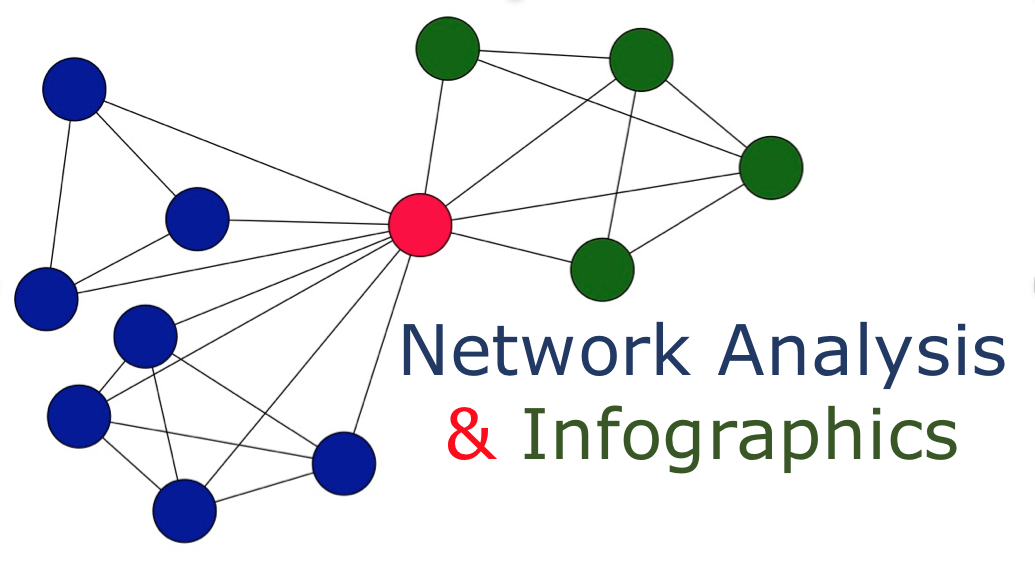
\includegraphics[width=2.5cm]{../_shared_pics/logo}

\medskip

\textit{{\color{dkgreen}{Week 4}}}\\
}


\date{} % Date, can be changed to a custom date

\begin{document}

\begin{frame}
\titlepage % Print the title page as the first slide

\begin{textblock*}{10pt}(0pt, 0.9\textheight)

\includegraphics[width=4cm]{../_shared_pics/SPRU.png}
\end{textblock*}

\end{frame}


%=======================================================
%	Learning outcomes
%=======================================================

\begin{frame}
\frametitle{Learning Outcomes}

\centering
\footnotesize
\begin{tabular}{lp{5.5cm}l}
\toprule
\multicolumn{2}{l}{\textbf{Learning outcome}} & \textbf{Assessment mode}\\
\hline
\\
1 & 
Explain the concept of network and list the main network indicators & 
ESS\\
\\
2 & 
Describe and apply the major techniques for the collection of network data and their statistical analysis & 
ESS, GPN + GWS\\
\\
\rowcolor{green!20}3 & 
Identify the main characteristics of networks by means of network measures  & 
ESS, GPN + GWS\\
\\
4 &
Employ network analysis techniques to produce network data-based infographics & 
GPN + GWS\\
\\
\bottomrule
\multicolumn{3}{l}{Note: ESS: Essay; GPN: Group Presentation; GWS: Group Written Submission}\\
\end{tabular}

\end{frame}

%------------------------------------------------




%=======================================================
%	Intro slides
%=======================================================
\section*{Overview}
%------------------------------------------------

\begin{frame}
\frametitle{\insertsection}
\tableofcontents
\end{frame}



%=======================================================
%	Approaches to the analysis of networks [recap]
%=======================================================
\section{Approaches to the analysis of networks [recap]}
%------------------------------------------------

\bgroup
\setbeamercolor{background canvas}{bg = navyblue}
\begin{frame}[plain]{}
\begin{center}
\color{white}{\Huge\insertsection}
\end{center}
\end{frame}
\egroup

%------------------------------------------------

\begin{frame}
\frametitle{\insertsection}


{\color{blue}{Descriptive network analysis}}\\ 
    \begin{itemize}
    \item An observed network is analysed by means of measures
    \item {\color{blue}{Network-level}} measures
    \item {\color{blue}{Node-level}} measures
    \end{itemize}

\bigskip
	
{\color{blue}{Modelling and inference of networks}}
    \begin{itemize}
    \item {\color{blue}{Mathematical models}}\\
    Based on `simple' probabilist rules to capture specific mechanisms (e.g.\ Erd\'os-R\'enyi networks, `the rich get richer')		
    \item {\color{blue}{Statistical models}}\\ 
    The observed network is considered as one of the possible realisation of a process -- a model that aims to fit to the observed data is specified (e.g.\ explanatory power of certain variables)
    \end{itemize}


\end{frame}

%------------------------------------------------

\begin{frame}
\frametitle{\insertsection}

Network Analysis is not a theory \textit{per se}, but it a methodological tool to support the development of theories \cite{Borgatti2011}

\begin{itemize}
    \item {\color{blue}{Network theory:}} mechanisms and processes that interact with network structures to produce certain outcomes for individuals, groups, and organisations (e.g.\ firms' performance, individuals' creativity)	
    
    \medskip
    
    \item {\color{blue}{Theory of networks:}} mechanisms and processes that explain why certain networks have certain structures (i.e.\ antecedents of network properties)
\end{itemize}

\medskip

\centering
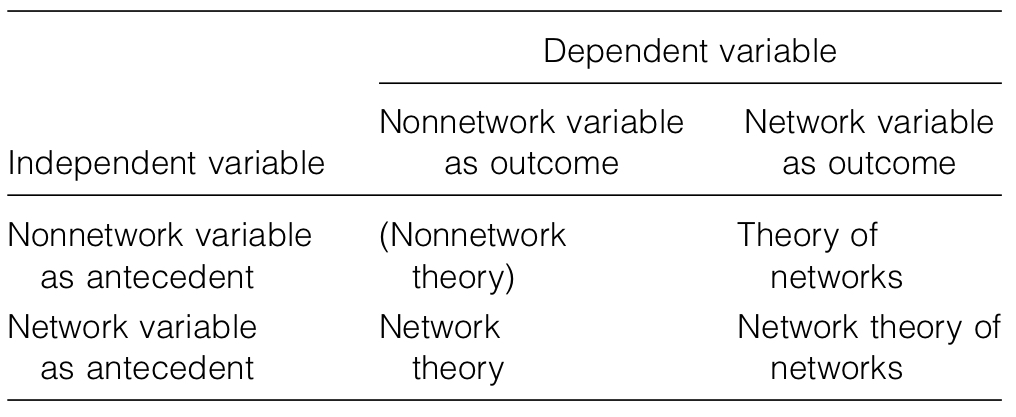
\includegraphics[width=6cm]{borgatti}\\
\tiny{Source: \cite{Borgatti2011}}
\end{frame}

%------------------------------------------------




%=======================================================
% Network-level measures
%=======================================================
\section{Network-level measures}
%------------------------------------------------

\bgroup
\setbeamercolor{background canvas}{bg = navyblue}
\begin{frame}[plain]{}
\begin{center}
\color{white}{\Huge\insertsection}
\end{center}
\end{frame}
\egroup

%------------------------------------------------

\begin{frame}
\frametitle{\insertsection}


\begin{columns}

\column{.45\textwidth} 
\begin{enumerate}
\item Diameter
\item Average Path Length (APL)
\item Density
\item Components
\item Cutpoints and bridges
\item Point/Line connectivity
\item Cliques
\item Inclusiveness
\item Reachable pairs
\item Transitivity
\end{enumerate}

\column{.45\textwidth} 
\onslide<2>{
\centering
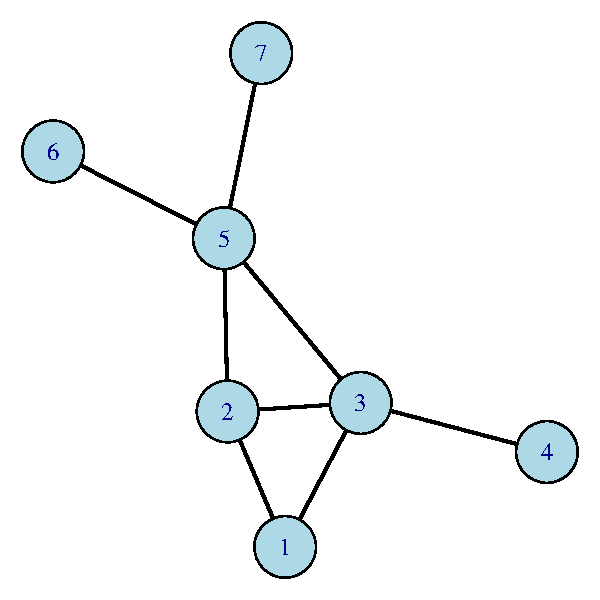
\includegraphics[width=5cm]{base}\\
\color{red}{\footnotesize Note: We will mostly focus on\\ undirected and unweighted networks}}

            
\end{columns}

\end{frame}

%------------------------------------------------
\subsection{Diameter}
%------------------------------------------------

\begin{frame}
\frametitle{\insertsection}
\framesubtitle{\insertsubsection}

\begin{columns}

\column{.45\textwidth} 
\begin{itemize}[<+->]
        \item To define the  {\color{blue}{diameter}} of a network, we need first to recall the definition of geodesic distance
        \item The {\color{blue}{geodesic distance}} between two nodes $n_i$ and $n_j$ is the shortest path* between these nodes
\end{itemize}

\column{.45\textwidth}
\centering
\only<1-2>{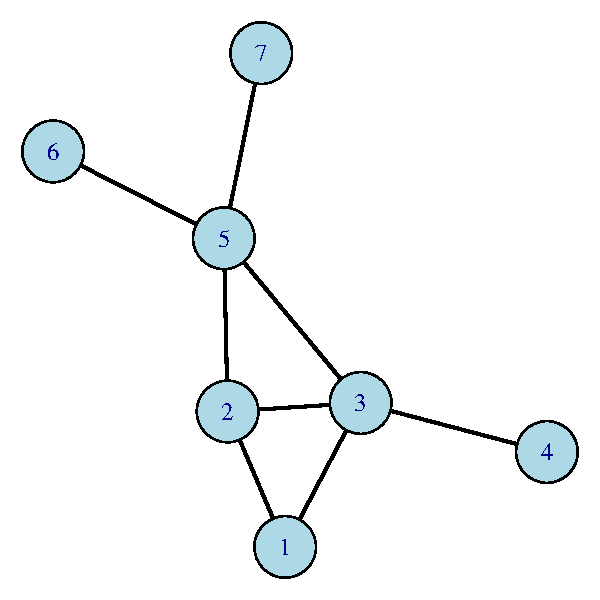
\includegraphics[width=5cm]{base}\\
$d(n_i, n_j)$}

\only<3>{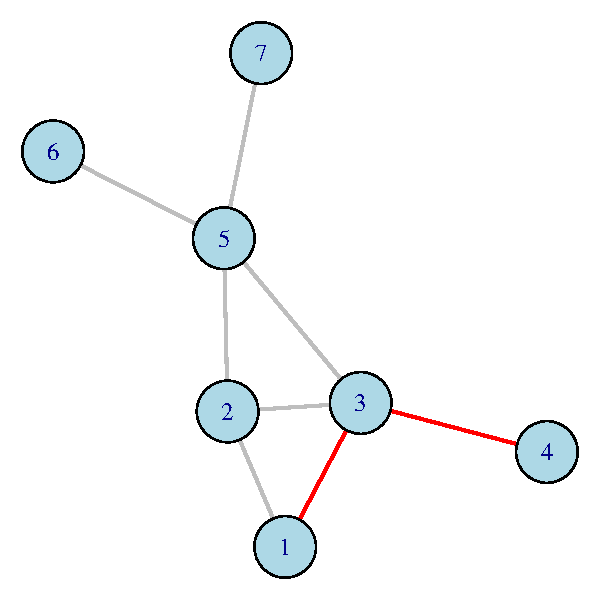
\includegraphics[width=5cm]{geodesic1}\\
$d(1,4)=2$}

\only<4>{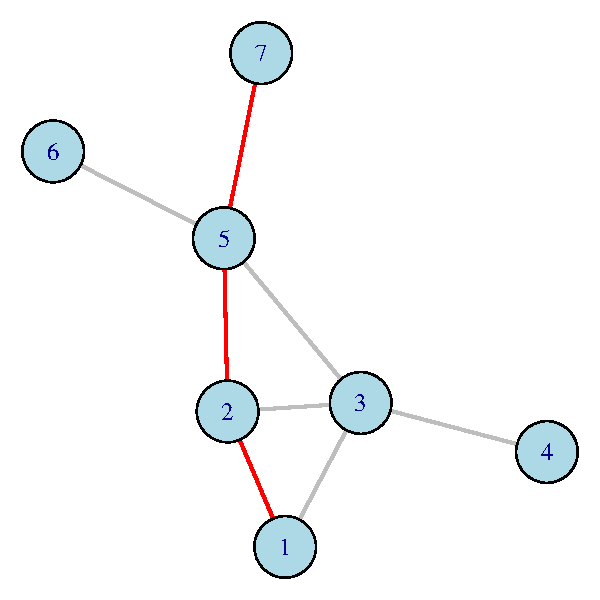
\includegraphics[width=5cm]{geodesic2}\\
$d(1,7)=3$}

\end{columns}


\only<2->{\begin{textblock*}{6cm}(1cm, 8cm)
\scriptsize{*A path is a sequence of nodes and lines (i.e.\ a walk) in which all nodes and links are distinct}
\end{textblock*}}


\end{frame}

%------------------------------------------------

\begin{frame}
\frametitle{\insertsection}
\framesubtitle{\insertsubsection}

\begin{columns}

\column{.45\textwidth} 
\begin{itemize}
\item The largest geodesic distance between any pair of nodes in a network is called {\color{blue}{diameter}}
\end{itemize}	

\begin{equation*}
D=max_i max_j d(n_i,n_j)
\end{equation*}

\begin{itemize}
\item The diameter of a network can range from $1$ to $N-1$
\end{itemize}

\column{.45\textwidth}
\centering
\only<1>{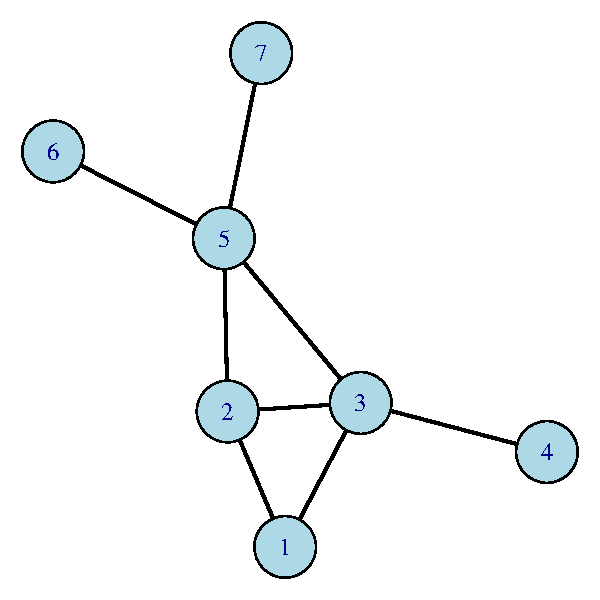
\includegraphics[width=5cm]{base}\\
            $D=max_i max_j d(n_i,n_j)$}
            
\only<2>{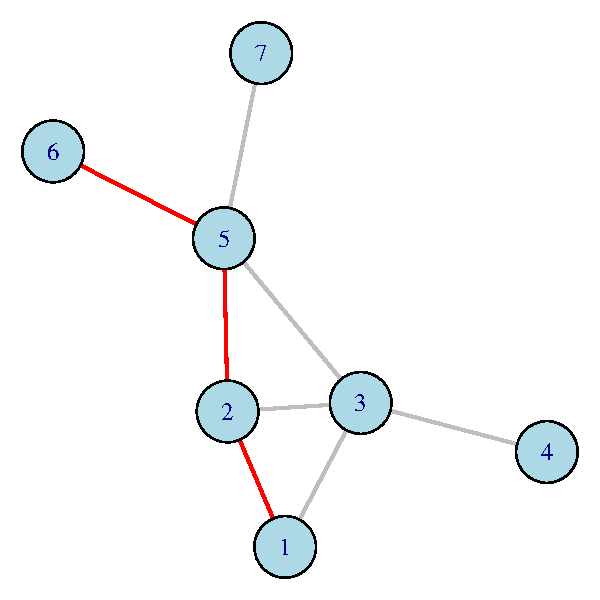
\includegraphics[width=5cm]{diameter}\\
            $D=3$}

\end{columns}

\end{frame}

%------------------------------------------------

\begin{frame}
\frametitle{\insertsection}
\framesubtitle{\insertsubsection}

\begin{columns}
\column{.45\textwidth} 

\footnotesize
\centering
\begin{tabular}{cc}
\toprule
Nodes & Geodesic distance\\
\hline
1-2 & 1\\
1-3 & 1\\
1-4 & 2\\
1-5 & 2\\
1-6 & 3\\
1-7 & 3\\
2-3 & 1\\
2-4 & 2\\
2-5 & 1\\
2-6 & 2\\
2-7 & 2\\
3-4 & 1\\
3-5 & 1\\
3-6 & 2\\
3-6 & 2\\
4-5 & 2\\
4-6 & 3\\
4-7 & 3\\
5-6 & 1\\
5-7 & 1\\
6-7 & 2\\
\bottomrule
\end{tabular}


\column{.45\textwidth}
\centering
\begin{overprint}
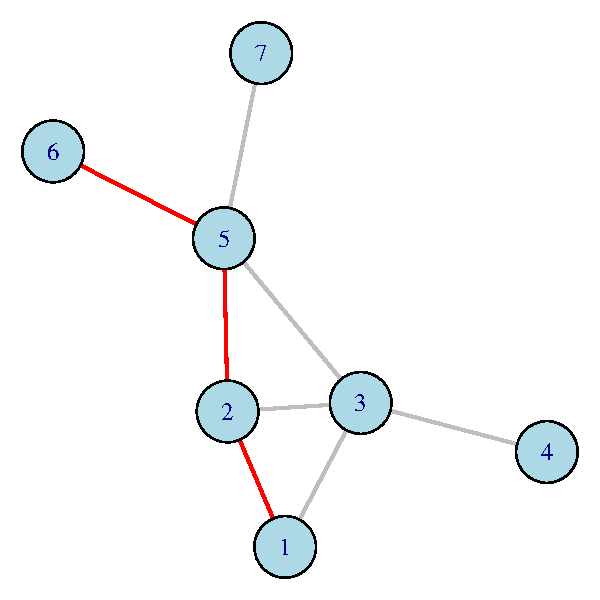
\includegraphics[width=5cm]{diameter}\\
            $D=max_i max_j d(n_i,n_j)=3$
\end{overprint}
            
\end{columns}

\end{frame}

%------------------------------------------------
\subsection{Average Path Length (APL)}
%------------------------------------------------

\begin{frame}
\frametitle{\insertsection}
\framesubtitle{\insertsubsection}

\begin{columns}
\column{.45\textwidth} 
\begin{itemize}
\item {\color{blue}{Average Path Length (APL)}} of a network is defined as
\end{itemize}

\begin{equation*}
APL = \frac{\sum_{n_i\neq n_j}d(n_i,n_j)}{\frac{N(N-1)}{2}}
\end{equation*}

\begin{itemize}
\item APL cannot be larger than the diameter of the network
\end{itemize}

\column{.45\textwidth}
\centering
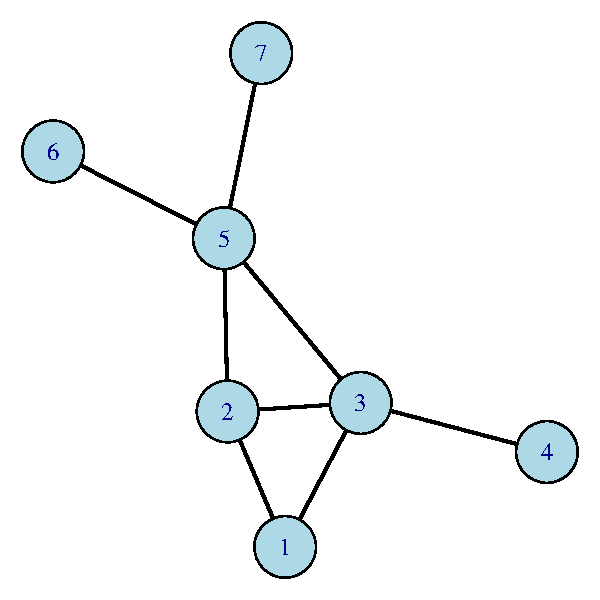
\includegraphics[width=5cm]{base}\\
        $APL = 38/21 = 1.81$
\end{columns}

\end{frame}

%------------------------------------------------
\subsection{Density}
%------------------------------------------------

\begin{frame}
\frametitle{\insertsection}
\framesubtitle{\insertsubsection}

\begin{columns}
\column{.45\textwidth} 
\begin{itemize}
	\item The {\color{blue}{density}} of a network is defined as number of edges in the network out the number of possible edges
\end{itemize}	

\begin{equation*}
\Delta=\frac{E}{\frac{N(N-1)}{2}}
\end{equation*}

\begin{itemize}
\item $N$ nodes, $E$ edges
\item The density of a network ranges from $0$ (no edges between nodes) to $1$ (fully-connected network)
\end{itemize}

\column{.45\textwidth}
\centering
\includegraphics<1>[width=5cm]{base}
\includegraphics<2>[width=5cm]{density1}
\includegraphics<3>[width=5cm]{density2}

\only<1>{$\Delta=\frac{8}{\frac{7(7-1)}{2}}=0.38$}
\only<2>{$\Delta=\frac{5}{\frac{5(5-1)}{2}}=0.5$}
\only<3>{$\Delta=\frac{10}{\frac{5(5-1)}{2}}=1.0$}
\end{columns}

\end{frame}

%------------------------------------------------

\begin{frame}[fragile]
\frametitle{\insertsection}
\framesubtitle{\insertsubsection}

{\color{red}{Warnings}} when using the density measure for comparison purposes
\begin{itemize}

\medskip

\item The density measure is {\color{blue}{dependent on the size of the network}} (larger networks are likely to be less dense, i.e.\ more sparse)

\medskip

\item Comparison between {\color{blue}{different types}} of networks (e.g.\  who knows whom vs.\ who has a love affair with whom in an academic department)

\end{itemize}

\end{frame}

%------------------------------------------------

\begin{frame}[fragile]
\frametitle{\insertsection}
\framesubtitle{Example: Diameter, APL, density}

\begin{columns}[c]

\column{.4\textwidth}
\begin{minipage}[c][.5\textheight][c]{\linewidth}


{\color{blue}{Karate}} data including the social network between members of a university karate club
\begin{itemize}
\item $N = 34$
\item $E = 78$
\item $Diameter = 13$
\item $APL = 2.41$
\item $\Delta = 0.14$
\end{itemize}

\medskip
\medskip

\lstinputlisting[language = R, firstline = 15, lastline = 26]{handouts_script/L4_script_handouts.R}
\end{minipage}	   


\column{.6\textwidth}
\begin{minipage}[c][.5\textheight][c]{\linewidth}
\centering
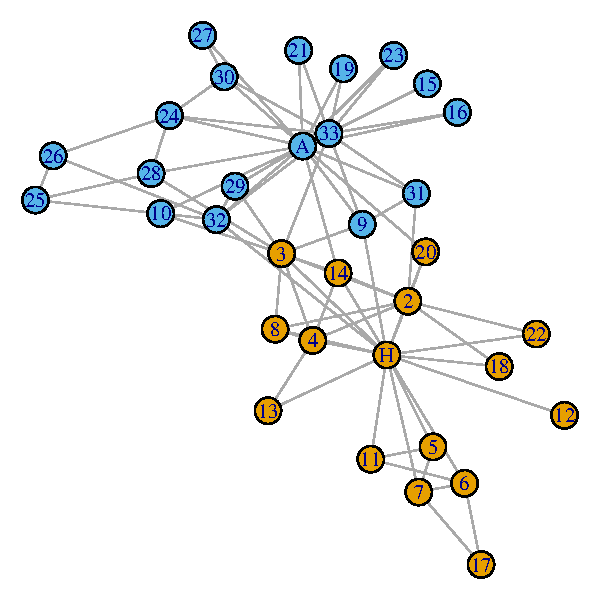
\includegraphics[height=0.7\textheight,keepaspectratio]{karate_density}\\
\tiny Source: \cite{Zachary1977}\\
\end{minipage}

\end{columns}

\end{frame}

%NOTE =============
%== Karate club network
%== Nodes represent members of a karate club
%== Ties are social interaction betweeen members
%== The clus split into two different clubs
%=================

%------------------------------------------------

\begin{frame}[fragile]
\frametitle{\insertsection}
\framesubtitle{Example: Diameter, APL, density}


\begin{columns}[c]

\column{.5\textwidth}
\begin{minipage}[c][.5\textheight][c]{\linewidth}

\medskip
\centering
\footnotesize The Godfather (1972)
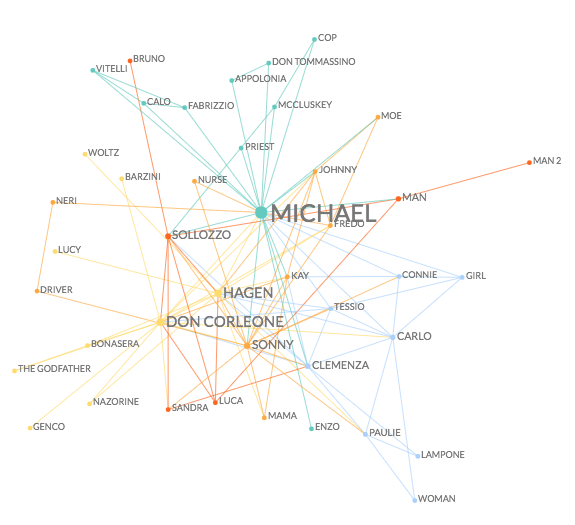
\includegraphics[width = 0.8\textwidth, keepaspectratio]{gf1}\\
\tiny Source: \url{http://moviegalaxies.com}

\footnotesize
\begin{itemize}
\item $N = 42$; $E = 104$
\item $Diameter = 4$; $APL = 2.26$; $\Delta = 0.12$
\end{itemize}

\lstinputlisting[language = R, firstline = 30, lastline = 34]{handouts_script/L4_script_handouts.R}
\end{minipage}	   

\column{.5\textwidth} 
\begin{minipage}[c][.5\textheight][c]{\linewidth}

\medskip
\centering
\footnotesize The Godfather (1974)
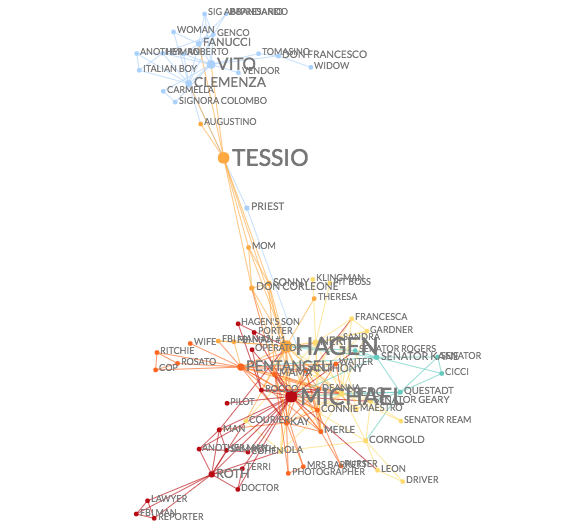
\includegraphics[width = 0.8\textwidth, keepaspectratio]{gf2}\\
\tiny Source: \url{http://moviegalaxies.com}

\footnotesize
\begin{itemize}
\item $N = 78$; $E = 219$
\item $Diameter = 7$; $APL = 3.06$; $\Delta = 0.07$
\end{itemize}

\lstinputlisting[language = R, firstline = 36, lastline = 40]{handouts_script/L4_script_handouts.R}
\end{minipage}	 

\end{columns}

\end{frame}


%------------------------------------------------
\subsection{Components}
%------------------------------------------------

\begin{frame}
\frametitle{\insertsection}
\framesubtitle{\insertsubsection}

\begin{columns}
\column{.45\textwidth} 
\begin{itemize}
	\item A {\color{blue}{component}} is a connected subgraph of a \textit{disconnected network}, i.e. a path between all pairs of nodes in the subgraph exists
	\item The number of components provides some indication about {\color{blue}{network connectivity}}
	\item The component with the largest number of nodes is called {\color{blue}{giant or largest component}}
	\item Network measures that are based on distances between nodes (e.g.\ APL) are assessed on the largest component of an disconnected network
\end{itemize}

\column{.45\textwidth}
\centering
\includegraphics<1>[width=5cm]{components1}
\includegraphics<2->[width=5cm]{components2}

\end{columns}

\end{frame}


%------------------------------------------------

\begin{frame}[fragile]
\frametitle{\insertsection}
\framesubtitle{\insertsubsection}

\begin{columns}[c]

\column{.5\textwidth}
\centering
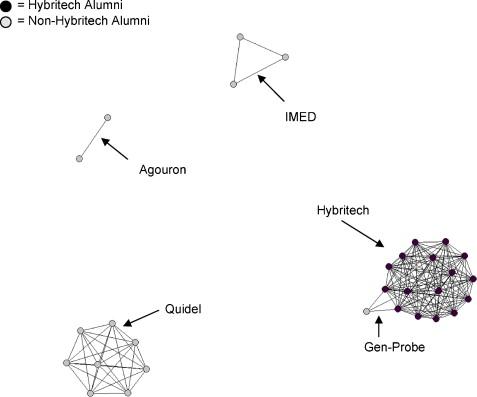
\includegraphics[width = 0.8\textwidth]{network_emergence_1}\\
\tiny Source: Career affiliation network, San Diego 1984 \cite{Casper2007}

\column{.5\textwidth}
\centering
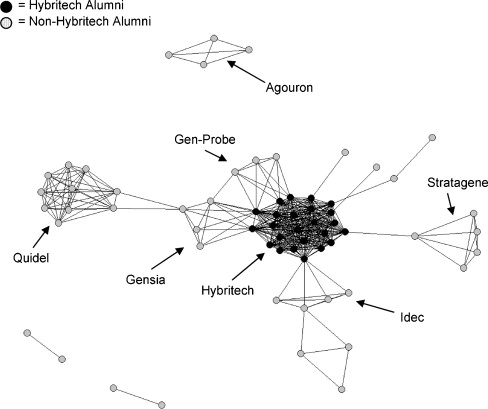
\includegraphics[width = 0.8\textwidth]{network_emergence_2}\\
\tiny Source: Career affiliation network, San Diego 1987 \cite{Casper2007}


\end{columns}

\end{frame}


% The article uses social network analysis to examine the emergence of social networks linking senior managers employed in biotechnology firms in San Diego, California
% The study examines the emergence of career affiliation networks formed between senior managers on the basis of ties between individuals that are formed through joint employment at the same organization 
% Early start-up company called Hybritech played a dominant role in seeding the development of two generations of successor companies in San Diego

%------------------------------------------------

\begin{frame}[fragile]
\frametitle{\insertsection}
\framesubtitle{\insertsubsection}

\begin{columns}[c]

\column{.5\textwidth}
\centering
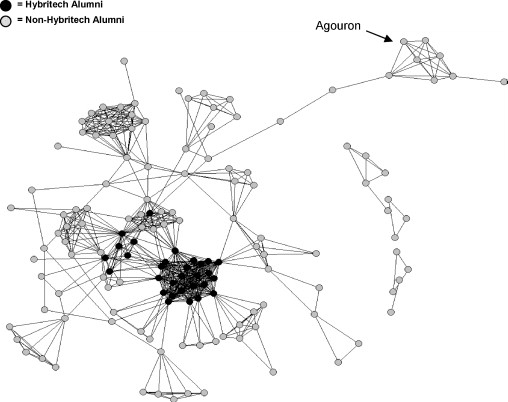
\includegraphics[width = 0.8\textwidth]{network_emergence_3}\\
\tiny Source: Career affiliation network, San Diego 1990 \cite{Casper2007}

\column{.5\textwidth}
\centering
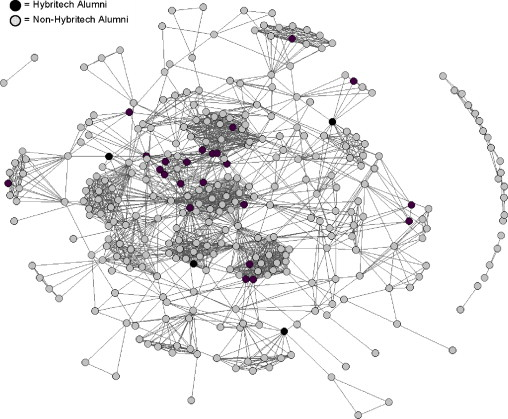
\includegraphics[width = 0.8\textwidth]{network_emergence_4}\\
\tiny Source: Career affiliation network, San Diego 1995 \cite{Casper2007}

\end{columns}

\end{frame}

%------------------------------------------------

\begin{frame}[fragile]
\frametitle{\insertsection}
\framesubtitle{\insertsubsection}

\centering
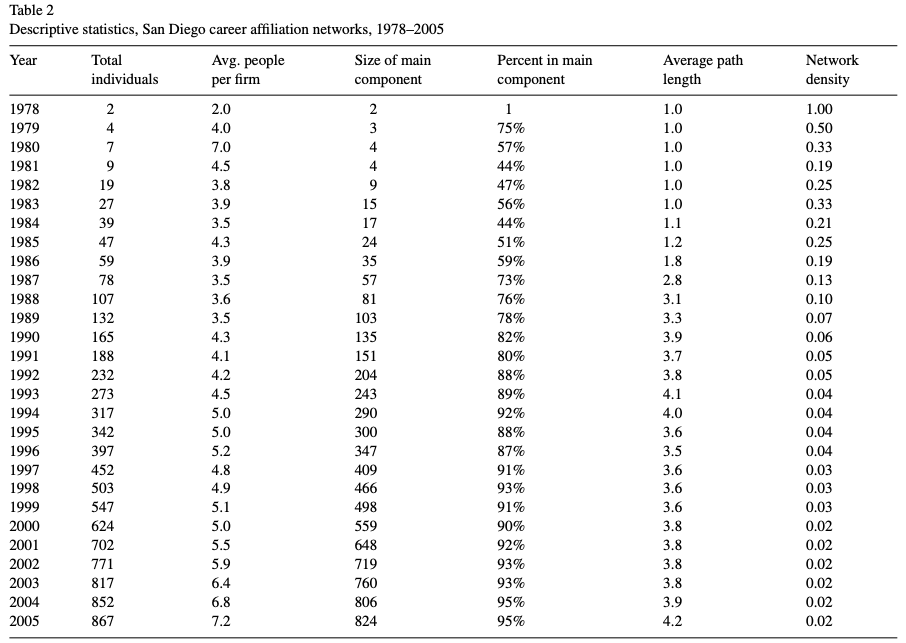
\includegraphics[width = 0.8\textwidth]{network_emergence_table}\\
\tiny Source: \cite{Casper2007}

\end{frame}

%------------------------------------------------



%------------------------------------------------
\subsection{Cutpoints and bridges}
%------------------------------------------------

\begin{frame}
\frametitle{\insertsection}
\framesubtitle{\insertsubsection}

\begin{columns}
\column{.45\textwidth} 
\begin{itemize}[<+->]
	\item <1,2,3,4> A {\color{blue}{cutpoint}} is a node the removal of which increases the number of components
	\item <3,4> A {\color{blue}{bridge}} is a link the removal of which increases the number of components 
\end{itemize}

\column{.45\textwidth}
\centering
\includegraphics<1>[width=5cm]{components2}
\includegraphics<2>[width=5cm]{cutpoint}
\includegraphics<3>[width=5cm]{components2}
\includegraphics<4>[width=5cm]{bridge}

\end{columns}

\end{frame}

%------------------------------------------------

\begin{frame}[fragile]
\frametitle{\insertsection}
\framesubtitle{\insertsubsection}

\centering
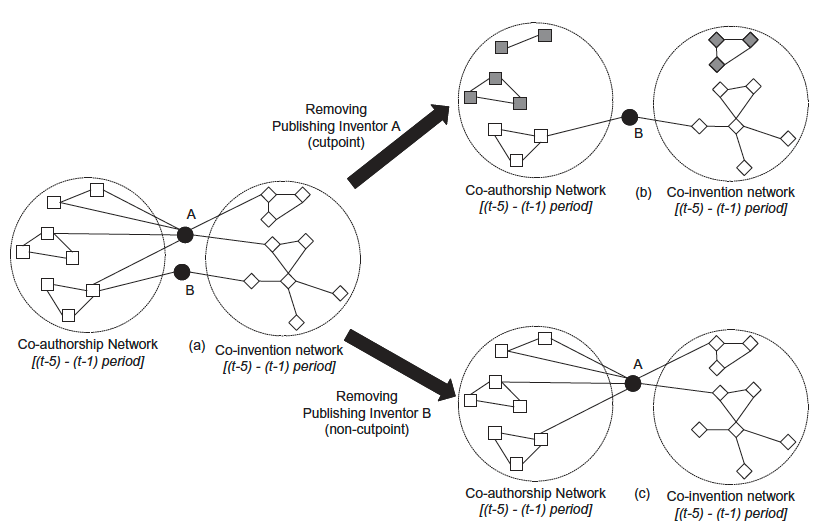
\includegraphics[width = 0.8\textwidth]{cattani}\\
\tiny Source: \cite{Cattani2013}

\end{frame}

%------------------------------------------------

\begin{frame}
\frametitle{\insertsection}
\framesubtitle{\insertsubsection}

\begin{columns}

\column{.4\textwidth}

\centering
\footnotesize
\begin{table}
\begin{tabular}{cl}
\bottomrule
\textbf{R\&D project} & \textbf{List of partners}\\
\hline
Proj01          & U2, F1, NG1\\
Proj02          & U1, NG4, F1\\
Proj03          & NG3, NG1, F1\\
Proj04          & NG3, NG4, F1\\
Proj05          & U3, F1\\
Proj06          & U3, F2\\
Proj07          & U3, F3\\
Proj08          & U3, U4\\
Proj09          & F1\\
Proj10          & U5\\
Proj11          & U4, U5, U6\\
Proj12          & U3, U7\\
Proj13          & U7, G1\\
Proj14          & U7, O1\\
Proj15          & U7, G2\\
Proj16          & G2, F3\\
Proj17          & F3, O2\\
Proj18          & O2, F4, NG2\\
Proj19          & F4, U9, NG2\\
Proj20          & NG2, U8\\
\bottomrule
\multicolumn{2}{l}{\tiny Firm (F); University (U); Gov. org. (G);}\\
\multicolumn{2}{l}{\tiny Non-Gov. org. (NG); Other (O)}
\end{tabular}
\end{table}



\column{.60\textwidth}
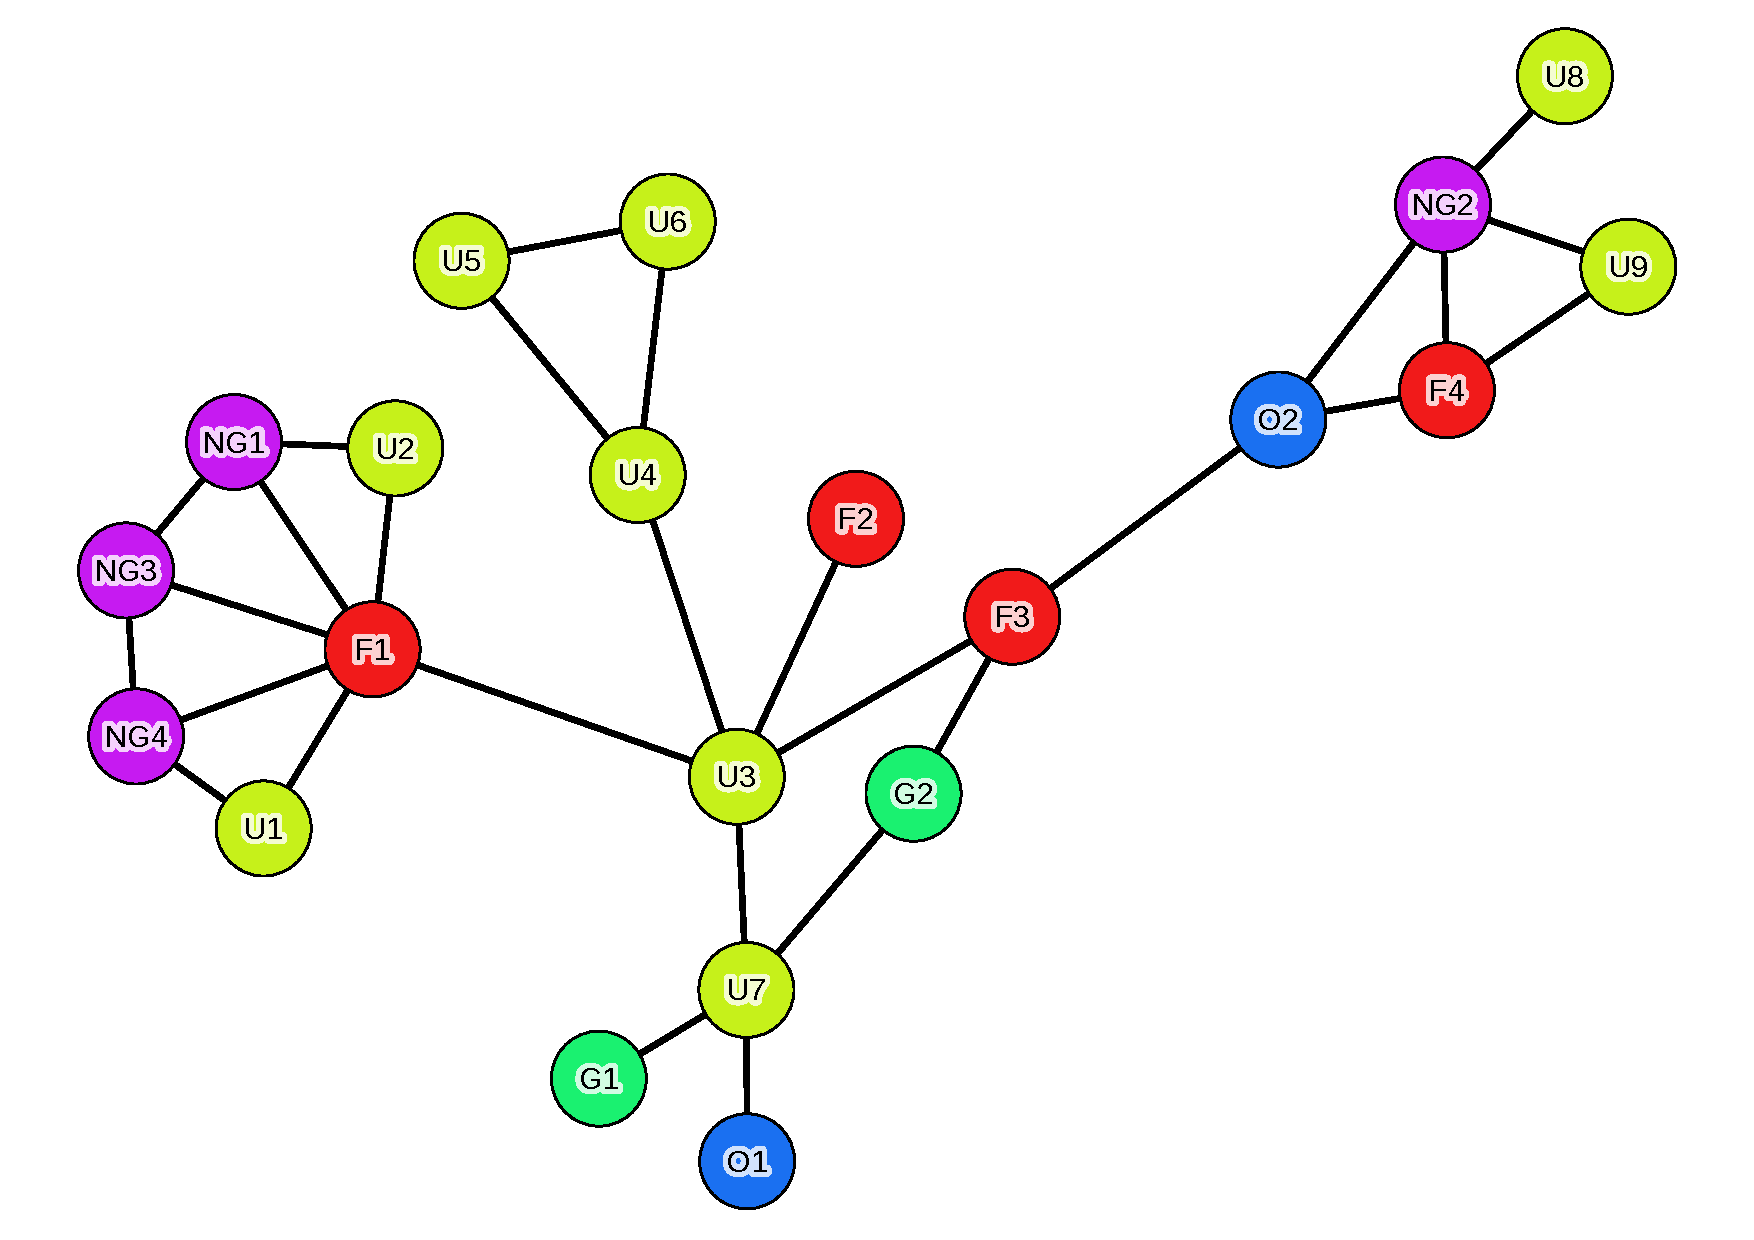
\includegraphics[width=\linewidth]{exercise_gephi}

\begin{itemize}
\item Which nodes are cutpoints?\\
\item How many bridges exist?
\end{itemize}  

\end{columns}

\end{frame}


%------------------------------------------------
\subsection{Connectivity}
%------------------------------------------------

\begin{frame}
\frametitle{\insertsection}
\framesubtitle{\insertsubsection: Point-connectivity}

\begin{columns}[c]

\column{.45\textwidth}
\begin{minipage}[c][.5\textheight][c]{\linewidth}

\begin{itemize}[<+->]
	\item The {\color{blue}{point-connectivity}} of a network is the minimum number of nodes we need to remove to make the network disconnected
	\item If the network is disconnected: $k=0$
	\item If the network includes at least one cutpoint: $k=1$
	\item If we need to remove at least two nodes to disconnect the network: $k=2$
\end{itemize}

\end{minipage}	   


\column{.6\textwidth}
\begin{minipage}[c][.5\textheight][c]{\linewidth}
\centering
\only<2>{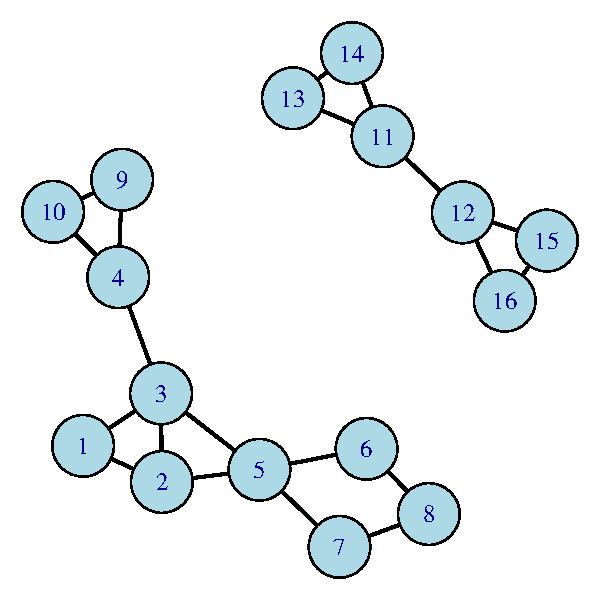
\includegraphics[width=5cm]{components1}}
\only<3>{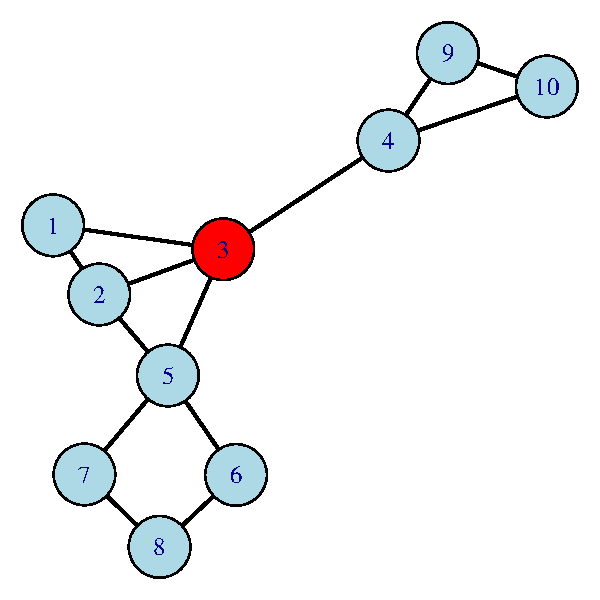
\includegraphics[width=5cm]{point_connectivity1}}
\only<4>{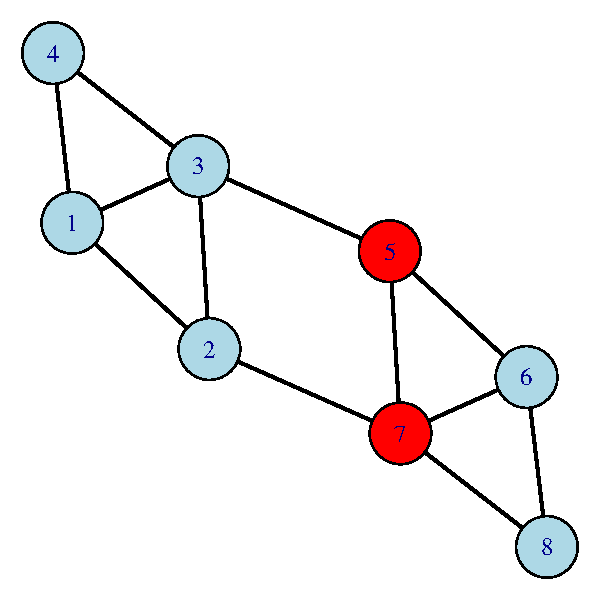
\includegraphics[width=5cm]{point_connectivity2}}
\end{minipage}	 

\end{columns}

\end{frame}

%------------------------------------------------

\begin{frame}
\frametitle{\insertsection}
\framesubtitle{\insertsubsection: Line-connectivity}

\begin{columns}[c]

\column{.45\textwidth}
\begin{minipage}[c][.5\textheight][c]{\linewidth}

\begin{itemize}[<+->]
	\item The {\color{blue}{line-connectivity}} of a network is the minimum number of lines/edges we need to remove to disconnect the network
	\item If the network is disconnected: $l=0$
	\item If the network includes one bridge: $l=1$
	\item If we need to remove at least two lines to disconnect the network: $l=2$
\end{itemize}

\end{minipage}	   

\column{.6\textwidth}
\begin{minipage}[c][.5\textheight][c]{\linewidth}
\centering
\only<2>{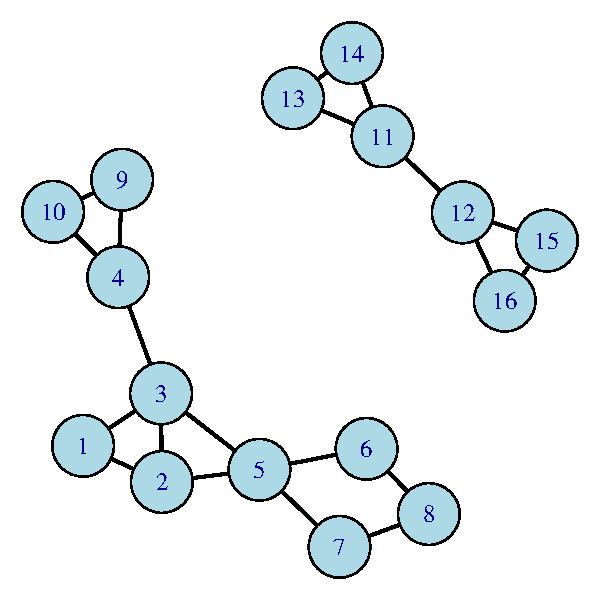
\includegraphics[width=5cm]{components1}}
\only<3>{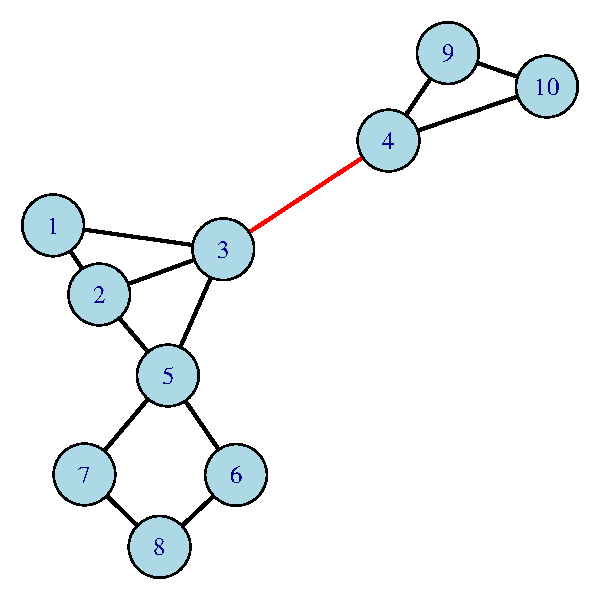
\includegraphics[width=5cm]{line_connectivity1}}
\only<4>{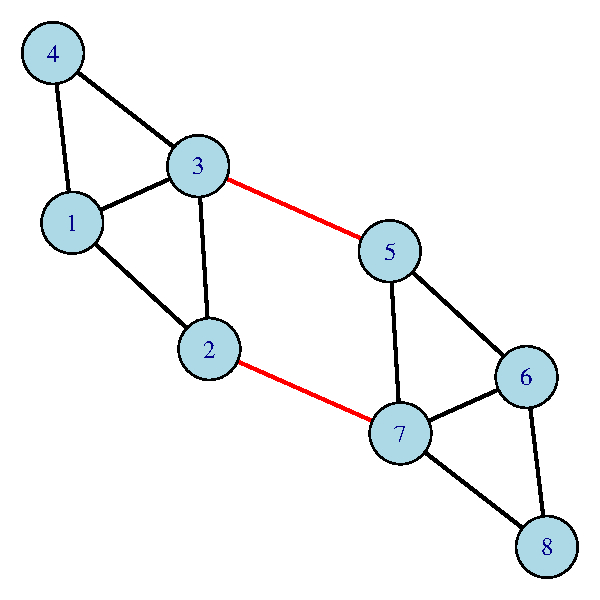
\includegraphics[width=5cm]{line_connectivity2}}
\end{minipage}	 

\end{columns}

\end{frame}

%------------------------------------------------
\subsection{Cliques}
%------------------------------------------------

\begin{frame}
\frametitle{\insertsection}
\framesubtitle{\insertsubsection}

\begin{columns}
\column{.45\textwidth} 
\begin{itemize}[<+->]
	\item<1-> A {\color{blue}{clique}} is a subgraph of three or more nodes where ties exist between every pair of nodes (maximal complete subgraph)
	\item<4,5>An {\color{blue}{n-clique}} is a subgraph with largest geodesic distance between any pair of nodes not larger than $n$
\end{itemize}

\column{.45\textwidth}
\centering
\includegraphics<1>[width=5cm]{base}
\includegraphics<2>[width=5cm]{clique1}
\includegraphics<3>[width=5cm]{clique2}
\includegraphics<4>[width=5cm]{base}
\includegraphics<5>[width=5cm]{clique3}

\end{columns}

\end{frame}

%------------------------------------------------
\subsection{Inclusiveness}
%------------------------------------------------

\begin{frame}
\frametitle{\insertsection}
\framesubtitle{\insertsubsection}

\begin{columns}
\column{.45\textwidth} 
\begin{itemize}[<+->]
	\item {\color{blue}{Inclusiveness}} is a defined as the number of connected nodes out the total number of nodes in a  network
	\item Nodes that have no ties are called {\color{blue}{isolates}}
\end{itemize}

\column{.45\textwidth}
\centering
\only<1>{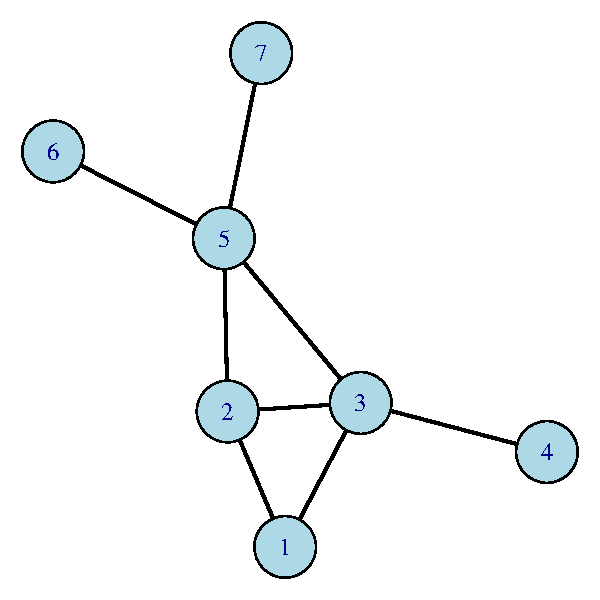
\includegraphics[width=5cm]{base}\\
        $inclusiveness = 7/7 = 1.00$}
\only<2>{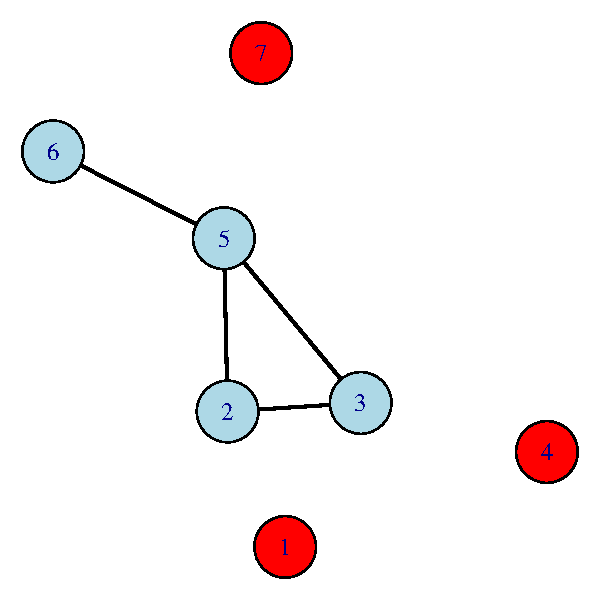
\includegraphics[width=5cm]{inclusiveness}\\
        $inclusiveness = 4/7 = 0.57$}

\end{columns}

\end{frame}

%------------------------------------------------
\subsection{Reachable pairs}
%------------------------------------------------

\begin{frame}
\frametitle{\insertsection}
\framesubtitle{\insertsubsection}

\begin{columns}
\column{.45\textwidth} 
\begin{itemize}
	\item Two nodes are {\color{blue}{reachable}} if a path between them exists (this property is called {\color{blue}{reachability}})
	\item The number of reachable node pairs out the total number of node pairs would provide an indication of {\color{blue}{network connectivity}}
	\item Geodesic distance matrix
\end{itemize}

\column{.45\textwidth}
\centering
\only<1>{\centering
        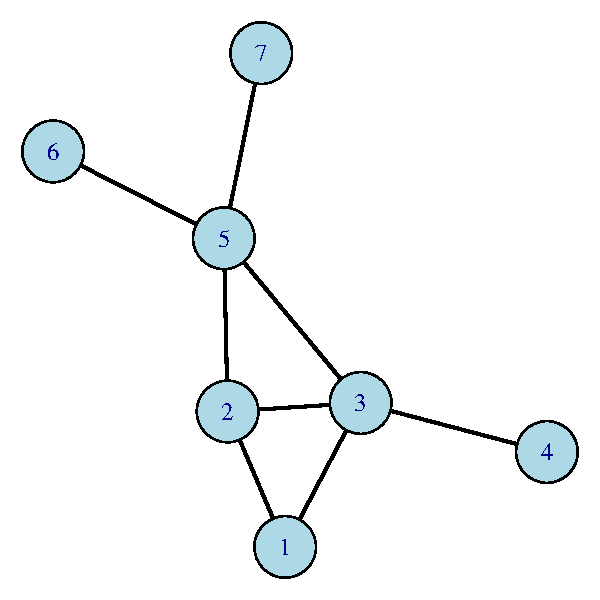
\includegraphics[width=4cm]{base}\\
        \scriptsize{
        \[\mathbf{D} =\left(\begin{array}{@{}ccccccc@{}}
        - & . & . & . & . & . & .\\
        1 & - & . & . & . & . & .\\
        1 & 1 & - & . & . & . & .\\
        2 & 2 & 1 & - & . & . & .\\
        2 & 1 & 1 & 2 & - & . & .\\
        3 & 2 & 2 & 3 & 1 & - & .\\
        3 & 2 & 2 & 3 & 1 & 2 & -\\
        \end{array}\right)\]

        
        $21/21 = 1.00$}}
\only<2>{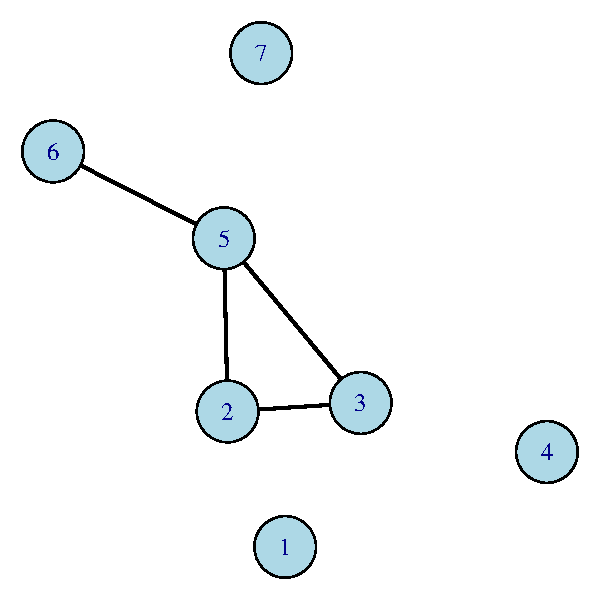
\includegraphics[width=4cm]{reachability}\\
        \scriptsize{
        \[\mathbf{D} =\left(\begin{array}{@{}ccccccc@{}}
        - & .  & .      & .      & . & . & .\\
        \infty & -      & .      & . & . & . & \\
        \infty & 1      & -      & . & . & . & .\\
        \infty & \infty & \infty & - & . & . & .\\
        \infty & 1      & 1 & \infty & - & . & .\\
        \infty & 2      & 2 & \infty & 1 & - & .\\
        \infty & \infty & \infty & \infty & \infty & \infty & -\\
        \end{array}\right)\]
        
        $6/21 = 0.28$}}

\end{columns}

\end{frame}

%------------------------------------------------
\subsection{Transitivity}
%------------------------------------------------

\begin{frame}
\frametitle{\insertsection}
\framesubtitle{\insertsubsection}

\begin{columns}
\column{.45\textwidth} 
\begin{itemize}
\item {\color{blue}{Transitivity}} is defined as the number of \textit{closed triads} out the number of \textit{closed} and \textit{open triads}
\item Closed triad: 
    \begin{itemize}
    \item $n_i \leftrightarrow n_j$
    \item $n_j \leftrightarrow n_k$
    \item $n_i \leftrightarrow n_k$
    \end{itemize}
    
\item Open triad : 
    \begin{itemize}
    \item $n_i \leftrightarrow n_j$
    \item $n_j \leftrightarrow n_k$
    \item no tie between $n_i$ and $n_k$
    \end{itemize}
\end{itemize}

\column{.45\textwidth}
\centering
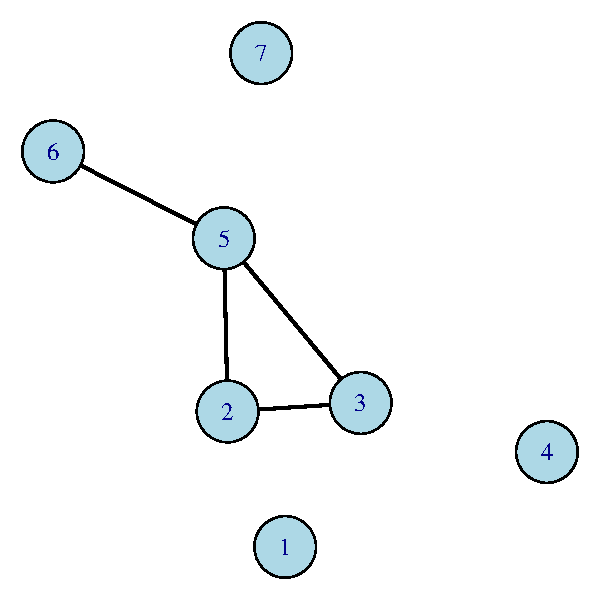
\includegraphics[width=5cm]{reachability}\\
$Transitivity = 3/5 = 0.60$

\end{columns}

\end{frame}

%------------------------------------------------

\begin{frame}
\frametitle{\insertsection}
\framesubtitle{Exercise}

\begin{columns}

\column{.45\textwidth} 

Characterise the network in terms of
\begin{itemize}
\item Diameter
\item APL
\item Components
\item Cutpoints
\item Transivity
\end{itemize}

\column{.45\textwidth}
\centering
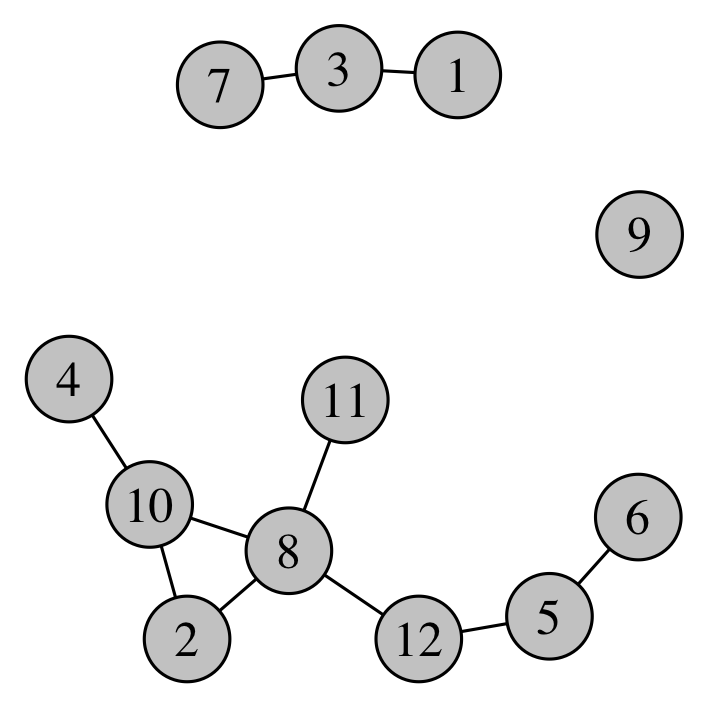
\includegraphics[width=5cm]{exercise.png}

\end{columns}

\end{frame}

%Diameter = 5
%APL = 2.23
%Components = 3
%Cutpoints = 5 (nodes 3, 5, 8, 10, 12)
%Transitivity = 0.23 (3 closed / (3 closed + 10 open)
%7-3-1	12-5-6	5-12-8	2-8-11 2-8-12 10-8-12 11-8-10 11-8-12 4-10-2 4-10-8


%------------------------------------------------

\begin{frame}
\frametitle{\insertsection}
\framesubtitle{Summary}

\footnotesize
\centering
\begin{tabular}{p{3cm}p{7.5cm}}
\toprule
\textbf{Measure} & \textbf{Interpretation}\\
\hline
\\
Diameter                        & Maximum time/resources for communication, transfer, ...\\
\\
APL                             & Average time/resources for communication, transfer, ...\\
\\
Density                         & Connectivity of a network \\
\\
Components                      & Presence of unconnected groups, bridging opportunities, ... \\
\\
Cutpoints and bridges           & Vulnerability/resilience of a network\\
\\
Point/Line connectivity         & Vulnerability/resilience of a network\\
\\
Cliques                         & Highly connected sub-groups, exclusion, ...\\
\\
Inclusiveness                   & Presence of unconnected nodes, exclusion, ... \\    
\\
Reachable pairs                 & Unconnected nodes or groups, bridging opportunities, ... \\
\\
Transitivity                    & Social interactions, `friends of my friends are my friends', ... \\

\bottomrule
\end{tabular}

\end{frame}


%=======================================================
%	Questions
%=======================================================
\bgroup
\setbeamercolor{background canvas}{bg = orange}
\begin{frame}[plain]{}
\begin{center}
\color{white}{\Huge Questions}
\end{center}
\end{frame}
\egroup
  

%%=======================================================
%	Next time ...
%%=======================================================
\section*{Next time ...}

%------------------------------------------------

\bgroup
\setbeamercolor{background canvas}{bg = navyblue}
\begin{frame}[plain]{}
\begin{center}
\color{white}{\Huge\insertsection}
\end{center}
\end{frame}
\egroup

%------------------------------------------------

\begin{frame}
\frametitle{\insertsection}

\begin{itemize}

\item 	\textbf{Seminar: Descriptive network analysis A}
	\begin{itemize}
	\item Assessment of network-level measures in igraph
	\end{itemize}	
	

\medskip
\medskip

\item 	\textbf{Lecture: Descriptive network analysis B}
	\begin{itemize}
	\item Node-level measures (centrality measures)
	\end{itemize}
	
	

		
\end{itemize}

\end{frame}

%------------------------------------------------





%=======================================================
%	References
%=======================================================
\begin{frame}[allowframebreaks]
\frametitle{References}
\tiny
\bibliographystyle{apalike}
\bibliography{references(2).bib}
\end{frame}
%------------------------------------------------




\end{document}